\section{Summary}
%================
\subsection{Specified and measured responses}
%--------------------------------------------
The NPP ATMS specified central frequencies, sideband offsets and channel bandwidths, taken from table 9 of the CrIS EDR ATBD\cite{CrIS_EDR_ATBD}, are shown in table \ref{tab:atms_fo_sb_and_df}. Also shown 
are measured bandwidths taken from table 12-1 of the ATMS PFM Calibration Data Book\cite{ATMS_PFM_CalLog}. No measurements of the central frequencies are readily available \footnote{These values may be available in other ATMS reports, particularly: RE-13680 K/Ka Band Receiver Shelf Verification Report, RE-13658 W Band Receiver Shelf Verification Report, RE-13741 V Band Receiver Shelf Verification Report, and RE-13802 G Band Receiver Shelf Verification Report.}. These frequency parameters are used to construct the so-called ``boxcar'' spectral response functions. 

Note that the bandpass information presented in Table VII of the ATMS Receiver Specification\cite{ATMS_Receiver_Spec} is not used here because the sideband frequency offset for channel 17 ($\pm$1500MHz) is  incorrect. Because no supplemental passband information from the referenced Table VII\cite{ATMS_Receiver_Spec} was used, channels 10 and 17 appear as single passband channels in table \ref{tab:atms_fo_sb_and_df}.

\begin{table}[htp]
  \centering
  \begin{tabular}{c c c c c c}
    \hline
                     & \textbf{Central}         & \textbf{Sideband 1}   & \textbf{Sideband 2}   & \textbf{Specified}       & \textbf{Measured} \\
                     & \textbf{Frequency}\up{a} & \textbf{Offset}\up{a} & \textbf{Offset}\up{a} & \textbf{Bandwidth}\up{a} & \textbf{Bandwidth}\up{b} \\
    \textbf{Channel} & \bfrequency{0}           & \bsideband{1}         & \bsideband{2}         & \bdeltaf                 & \bdeltaf      \\
                     & (GHz)                    & (GHz)                 & (GHz)                 & (GHz)                    & (GHz)         \\
    \hline\hline
            1        &  23.800000  & -      & -      & 0.27   & 0.258         \\
            2        &  31.400000  & -      & -      & 0.18   & 0.172         \\
            3        &  50.300000  & -      & -      & 0.18   & 0.173         \\
            4        &  51.760000  & -      & -      & 0.40   & 0.381         \\
            5        &  52.800000  & -      & -      & 0.40   & 0.366         \\
            6        &  53.596000  & 0.115  & -      & 0.17   & 0.1587,0.1648\up{c} \\
            7        &  54.400000  & -      & -      & 0.40   & 0.387         \\
            8        &  54.940000  & -      & -      & 0.40   & 0.387         \\
            9        &  55.500000  & -      & -      & 0.33   & 0.317         \\
           10        &  57.290344  & -      & -      & 0.33   & 0.151         \\
           11        &  57.290344  & 0.217  & -      & 0.078  & 0.0763        \\
           12        &  57.290344  & 0.3222 & 0.048  & 0.036  & 0.0351        \\
           13        &  57.290344  & 0.3222 & 0.022  & 0.016  & 0.01547       \\
           14        &  57.290344  & 0.3222 & 0.010  & 0.008  & 0.0078,0.0079\up{c} \\
           15        &  57.290344  & 0.3222 & 0.0045 & 0.003  & 0.0029        \\
           16        &  88.200000  & -      & -      & 2.0    & 1.9282        \\
           17        & 165.500000  & -      & -      & 3.0    & 1.1251        \\
           18        & 183.310000  & 7.0    & -      & 2.0    & 1.9302        \\
           19        & 183.310000  & 4.5    & -      & 2.0    & 1.9519        \\
           20        & 183.310000  & 3.0    & -      & 1.0    & 0.9799        \\
           21        & 183.310000  & 1.8    & -      & 1.0    & 0.9823        \\
           22        & 183.310000  & 1.0    & -      & 0.5    & 0.4940        \\
    \hline
  \end{tabular}
  \caption{Central, sideband offset, and bandwidth frequencies for ATMS. \superscript{a}Data from table 9 of ref.\cite{CrIS_EDR_ATBD}. \superscript{b}Data from table 12-1 of ref.\cite{ATMS_PFM_CalLog}. \superscript{c}Different lower and upper sideband widths reported. }
  \label{tab:atms_fo_sb_and_df}
\end{table}



\subsection{Selected testing conditions}
%---------------------------------------
Three temperatures were available for all the received data files, corresponding to the ``usual'' nominal, low, and high operating temperatures; in this case 20\textdegree{}C, -10\textdegree{}C, and 50\textdegree{}C respectively.

In addition to the temperature datasets, three bias voltages were also represented in the data: nominal, high, and low.

No thresholds were applied to any of the ATMS SRF data. Plots of the SRF data used for each test temperature and bias voltage for each channel are shown in appendices \ref{app:Tset} and \ref{app:Vset} respectively.


\subsection{Variable temperature SRF processing}
%-----------------------------------------------
The following tables list the computed central frequencies and polychromatic correction coefficients for the three test temperatures for the nominal bias voltage. The temperature fit residuals for each temperature and each channel are shown in appendix \ref{app:Tset_tfit_data_plots}.

Plots summarising these differences in the central frequencies and polychromatic correction coefficients for the low and high test temperature SRF datasets compared to the nominal temperature SRFs are shown in figure \ref{fig:Tset.summary}

\begin{figure}[H]
  \label{fig:Tset.summary}
  \centering
  \includegraphics[scale=0.7]{graphics/summary/atms_npp.Tset.summary.eps}
  \caption{Diffrences in the ATMS central frequencies (top) and polychromatic correction coefficients (middle, bottom) for the low (-10\textdegree{}C) and high (50\textdegree{}C) temperatures compared to the nominal (20\textdegree{}C) test temperature.}
\end{figure}

\begin{table}[htp]
  \centering
  \begin{tabular}{C{1.5cm} R{1.0cm}@{.}L{1.5cm} *{2}{R{1cm}@{.}L{2cm}}}
    \hline
    \sffamily{ATMS} & \multicolumn{2}{c}{$f_0$} & \multicolumn{2}{c}{$a_0$ (offset)} & \multicolumn{2}{c}{$a_1$ (slope)} \\
    \sffamily{Channel} & \multicolumn{2}{c}{\sffamily{(GHz)}} & \multicolumn{2}{c}{\sffamily{(K)}} & \multicolumn{2}{c}{\sffamily{(K/K)}}  \\
    \hline\hline
     1 &  23&795485 & -0&00001855 & 1&00001087 \\
     2 &  31&392329 & -0&00000572 & 1&00000254 \\
     3 &  50&299184 & -0&00000356 & 1&00000099 \\
     4 &  51&772506 & -0&00001613 & 1&00000437 \\
     5 &  52&807280 & -0&00001547 & 1&00000410 \\
     6 &  53&582786 & -0&00002022 & 1&00000529 \\
     7 &  54&397080 & -0&00001594 & 1&00000411 \\
     8 &  54&941564 & -0&00001688 & 1&00000431 \\
     9 &  55&483558 & -0&00001023 & 1&00000258 \\
    10 &  57&290258 & -0&00001058 & 1&00000259 \\
    11 &  57&290258 & -0&00005919 & 1&00001449 \\
    12 &  57&290264 & -0&00013257 & 1&00003245 \\
    13 &  57&290231 & -0&00012904 & 1&00003158 \\
    14 &  57&290223 & -0&00012854 & 1&00003146 \\
    15 &  57&290259 & -0&00012914 & 1&00003161 \\
    16 &  88&158114 & -0&00023173 & 1&00003703 \\
    17 & 165&502000 & -0&00040445 & 1&00003486 \\
    18 & 183&303997 & -0&01806741 & 1&00141016 \\
    19 & 183&304000 & -0&00778513 & 1&00060763 \\
    20 & 183&303999 & -0&00332830 & 1&00025977 \\
    21 & 183&304000 & -0&00122373 & 1&00009551 \\
    22 & 183&304000 & -0&00040732 & 1&00003179 \\
    \hline
  \end{tabular}
  \caption{The computed ATMS channel central frequencies and polychromatic correction coefficients for the T\subscript{\sffamily{nominal}} SRF dataset at nominal bias voltage.}
  \label{tab:atms_Tnominal_results}
\end{table}

\begin{table}[H]
  \centering
  \begin{tabular}{C{1.5cm} R{1.0cm}@{.}L{1.5cm} *{2}{R{1cm}@{.}L{2cm}}}
    \hline
    \sffamily{ATMS} & \multicolumn{2}{c}{$f_0$} & \multicolumn{2}{c}{$a_0$ (offset)} & \multicolumn{2}{c}{$a_1$ (slope)} \\
    \sffamily{Channel} & \multicolumn{2}{c}{\sffamily{(GHz)}} & \multicolumn{2}{c}{\sffamily{(K)}} & \multicolumn{2}{c}{\sffamily{(K/K)}}  \\
    \hline\hline
     1 &  23&797976 & -0&00002044 & 1&00001198 \\
     2 &  31&394058 & -0&00000573 & 1&00000255 \\
     3 &  50&296455 & -0&00000358 & 1&00000100 \\
     4 &  51&779796 & -0&00001590 & 1&00000430 \\
     5 &  52&798879 & -0&00001636 & 1&00000434 \\
     6 &  53&576448 & -0&00001976 & 1&00000517 \\
     7 &  54&394170 & -0&00001581 & 1&00000407 \\
     8 &  54&943874 & -0&00001695 & 1&00000432 \\
     9 &  55&482323 & -0&00001007 & 1&00000254 \\
    10 &  57&290260 & -0&00001078 & 1&00000264 \\
    11 &  57&290260 & -0&00005942 & 1&00001454 \\
    12 &  57&290230 & -0&00013448 & 1&00003291 \\
    13 &  57&290276 & -0&00012978 & 1&00003176 \\
    14 &  57&290280 & -0&00012864 & 1&00003148 \\
    15 &  57&290257 & -0&00012903 & 1&00003158 \\
    16 &  88&199020 & -0&00022672 & 1&00003623 \\
    17 & 165&482000 & -0&00040728 & 1&00003511 \\
    18 & 183&304003 & -0&01813779 & 1&00141565 \\
    19 & 183&303999 & -0&00783888 & 1&00061182 \\
    20 & 183&304001 & -0&00334559 & 1&00026112 \\
    21 & 183&303999 & -0&00124594 & 1&00009725 \\
    22 & 183&304000 & -0&00040937 & 1&00003195 \\
    \hline
  \end{tabular}
  \caption{The computed ATMS channel central frequencies and polychromatic correction coefficients for the T\subscript{\sffamily{low}} SRF dataset at nominal bias voltage.}
  \label{tab:atms_Tlow_results}
\end{table}

\begin{table}[H]
  \centering
  \begin{tabular}{C{1.5cm} R{1.0cm}@{.}L{1.5cm} *{2}{R{1cm}@{.}L{2cm}}}
    \hline
    \sffamily{ATMS} & \multicolumn{2}{c}{$f_0$} & \multicolumn{2}{c}{$a_0$ (offset)} & \multicolumn{2}{c}{$a_1$ (slope)} \\
    \sffamily{Channel} & \multicolumn{2}{c}{\sffamily{(GHz)}} & \multicolumn{2}{c}{\sffamily{(K)}} & \multicolumn{2}{c}{\sffamily{(K/K)}}  \\
    \hline\hline
     1 &  23&795526 & -0&00001988 & 1&00001165 \\
     2 &  31&394221 & -0&00000631 & 1&00000281 \\
     3 &  50&303330 & -0&00000354 & 1&00000098 \\
     4 &  51&760695 & -0&00001579 & 1&00000427 \\
     5 &  52&801361 & -0&00001529 & 1&00000406 \\
     6 &  53&577185 & -0&00002032 & 1&00000531 \\
     7 &  54&399892 & -0&00001590 & 1&00000410 \\
     8 &  54&938490 & -0&00001680 & 1&00000428 \\
     9 &  55&485991 & -0&00001014 & 1&00000256 \\
    10 &  57&290256 & -0&00001054 & 1&00000258 \\
    11 &  57&290256 & -0&00005903 & 1&00001445 \\
    12 &  57&290299 & -0&00013026 & 1&00003188 \\
    13 &  57&290258 & -0&00012813 & 1&00003136 \\
    14 &  57&290254 & -0&00012851 & 1&00003145 \\
    15 &  57&290300 & -0&00012915 & 1&00003161 \\
    16 &  88&149967 & -0&00024583 & 1&00003929 \\
    17 & 165&492000 & -0&00041133 & 1&00003546 \\
    18 & 183&314002 & -0&01805228 & 1&00140890 \\
    19 & 183&314000 & -0&00778112 & 1&00060728 \\
    20 & 183&314004 & -0&00330948 & 1&00025829 \\
    21 & 183&314001 & -0&00121723 & 1&00009500 \\
    22 & 183&314001 & -0&00040840 & 1&00003187 \\
    \hline
  \end{tabular}
  \caption{The computed ATMS channel central frequencies and polychromatic correction coefficients for the T\subscript{\sffamily{high}} SRF dataset at nominal bias voltage.}
  \label{tab:atms_Thigh_results}
\end{table}



\subsection{Variable bias voltage SRF processing}
%------------------------------------------------
The following tables list the computed central frequencies and polychromatic correction coefficients for the three test bias voltages for the nominal temperature. The temperature fit residuals for each bias voltage and each channel are shown in appendix \ref{app:Vset_tfit_data_plots}.

Plots summarising these differences in the central frequencies and polychromatic correction coefficients for the low and high test bias voltage SRF datasets compared to the nominal bias voltage SRFs are shown in figure \ref{fig:Vset.summary}

\begin{figure}[H]
  \label{fig:Vset.summary}
  \centering
  \includegraphics[scale=0.7]{graphics/summary/atms_npp.Vset.summary.eps}
  \caption{Diffrences in the ATMS central frequencies (top) and polychromatic correction coefficients (middle, bottom) for the low and high bias voltages compared to the nominal test bias voltage temperature.}
\end{figure}

\begin{table}[htp]
  \centering
  \begin{tabular}{C{1.5cm} R{1.0cm}@{.}L{1.5cm} *{2}{R{1cm}@{.}L{2cm}}}
    \hline
    \sffamily{ATMS} & \multicolumn{2}{c}{$f_0$} & \multicolumn{2}{c}{$a_0$ (offset)} & \multicolumn{2}{c}{$a_1$ (slope)} \\
    \sffamily{Channel} & \multicolumn{2}{c}{\sffamily{(GHz)}} & \multicolumn{2}{c}{\sffamily{(K)}} & \multicolumn{2}{c}{\sffamily{(K/K)}}  \\
    \hline\hline
     1 &  23&795485 & -0&00001855 & 1&00001087 \\
     2 &  31&392329 & -0&00000572 & 1&00000254 \\
     3 &  50&299184 & -0&00000356 & 1&00000099 \\
     4 &  51&772506 & -0&00001613 & 1&00000437 \\
     5 &  52&807280 & -0&00001547 & 1&00000410 \\
     6 &  53&582786 & -0&00002022 & 1&00000529 \\
     7 &  54&397080 & -0&00001594 & 1&00000411 \\
     8 &  54&941564 & -0&00001688 & 1&00000431 \\
     9 &  55&483558 & -0&00001023 & 1&00000258 \\
    10 &  57&290258 & -0&00001058 & 1&00000259 \\
    11 &  57&290258 & -0&00005919 & 1&00001449 \\
    12 &  57&290264 & -0&00013257 & 1&00003245 \\
    13 &  57&290231 & -0&00012904 & 1&00003158 \\
    14 &  57&290223 & -0&00012854 & 1&00003146 \\
    15 &  57&290259 & -0&00012914 & 1&00003161 \\
    16 &  88&158114 & -0&00023173 & 1&00003703 \\
    17 & 165&502000 & -0&00040445 & 1&00003486 \\
    18 & 183&303997 & -0&01806741 & 1&00141016 \\
    19 & 183&304000 & -0&00778513 & 1&00060763 \\
    20 & 183&303999 & -0&00332830 & 1&00025977 \\
    21 & 183&304000 & -0&00122373 & 1&00009551 \\
    22 & 183&304000 & -0&00040732 & 1&00003179 \\
    \hline
  \end{tabular}
  \caption{The computed ATMS channel central frequencies and polychromatic correction coefficients for the V\subscript{\sffamily{nominal}} SRF dataset at nominal temperature.}
  \label{tab:atms_Vnominal_results}
\end{table}

\begin{table}[H]
  \centering
  \begin{tabular}{C{1.5cm} R{1.0cm}@{.}L{1.5cm} *{2}{R{1cm}@{.}L{2cm}}}
    \hline
    \sffamily{ATMS} & \multicolumn{2}{c}{$f_0$} & \multicolumn{2}{c}{$a_0$ (offset)} & \multicolumn{2}{c}{$a_1$ (slope)} \\
    \sffamily{Channel} & \multicolumn{2}{c}{\sffamily{(GHz)}} & \multicolumn{2}{c}{\sffamily{(K)}} & \multicolumn{2}{c}{\sffamily{(K/K)}}  \\
    \hline\hline
     1 &  23&797491 & -0&00001671 & 1&00000979 \\
     2 &  31&392530 & -0&00000570 & 1&00000253 \\
     3 &  50&299337 & -0&00000354 & 1&00000099 \\
     4 &  51&773064 & -0&00001613 & 1&00000436 \\
     5 &  52&807348 & -0&00001552 & 1&00000412 \\
     6 &  53&580427 & -0&00001993 & 1&00000521 \\
     7 &  54&397258 & -0&00001595 & 1&00000411 \\
     8 &  54&942383 & -0&00001679 & 1&00000428 \\
     9 &  55&484511 & -0&00001021 & 1&00000258 \\
    10 &  57&290258 & -0&00001058 & 1&00000259 \\
    11 &  57&290258 & -0&00005901 & 1&00001444 \\
    12 &  57&290224 & -0&00013275 & 1&00003249 \\
    13 &  57&290300 & -0&00012900 & 1&00003157 \\
    14 &  57&290231 & -0&00012852 & 1&00003145 \\
    15 &  57&290254 & -0&00012914 & 1&00003161 \\
    16 &  88&157782 & -0&00024009 & 1&00003837 \\
    17 & 165&502000 & -0&00040442 & 1&00003486 \\
    18 & 183&303998 & -0&01810165 & 1&00141283 \\
    19 & 183&304000 & -0&00775770 & 1&00060549 \\
    20 & 183&304002 & -0&00331693 & 1&00025888 \\
    21 & 183&304000 & -0&00122613 & 1&00009570 \\
    22 & 183&304001 & -0&00040795 & 1&00003184 \\
    \hline
  \end{tabular}
  \caption{The computed ATMS channel central frequencies and polychromatic correction coefficients for the V\subscript{\sffamily{low}} SRF dataset at nominal temperature.}
  \label{tab:atms_Vlow_results}
\end{table}

\begin{table}[H]
  \centering
  \begin{tabular}{C{1.5cm} R{1.0cm}@{.}L{1.5cm} *{2}{R{1cm}@{.}L{2cm}}}
    \hline
    \sffamily{ATMS} & \multicolumn{2}{c}{$f_0$} & \multicolumn{2}{c}{$a_0$ (offset)} & \multicolumn{2}{c}{$a_1$ (slope)} \\
    \sffamily{Channel} & \multicolumn{2}{c}{\sffamily{(GHz)}} & \multicolumn{2}{c}{\sffamily{(K)}} & \multicolumn{2}{c}{\sffamily{(K/K)}}  \\
    \hline\hline
     1 &  23&797634 & -0&00001671 & 1&00000979 \\
     2 &  31&392588 & -0&00000570 & 1&00000253 \\
     3 &  50&298725 & -0&00000356 & 1&00000099 \\
     4 &  51&772800 & -0&00001618 & 1&00000438 \\
     5 &  52&808362 & -0&00001546 & 1&00000410 \\
     6 &  53&580087 & -0&00001984 & 1&00000519 \\
     7 &  54&396096 & -0&00001592 & 1&00000410 \\
     8 &  54&941726 & -0&00001688 & 1&00000431 \\
     9 &  55&484758 & -0&00001020 & 1&00000258 \\
    10 &  57&290258 & -0&00001059 & 1&00000259 \\
    11 &  57&290258 & -0&00005913 & 1&00001447 \\
    12 &  57&290309 & -0&00013265 & 1&00003247 \\
    13 &  57&290200 & -0&00012897 & 1&00003157 \\
    14 &  57&290209 & -0&00012853 & 1&00003146 \\
    15 &  57&290271 & -0&00012915 & 1&00003161 \\
    16 &  88&147443 & -0&00023310 & 1&00003725 \\
    17 & 165&502000 & -0&00040565 & 1&00003497 \\
    18 & 183&304003 & -0&01803843 & 1&00140789 \\
    19 & 183&304001 & -0&00777934 & 1&00060717 \\
    20 & 183&304000 & -0&00332740 & 1&00025970 \\
    21 & 183&304000 & -0&00122567 & 1&00009566 \\
    22 & 183&303999 & -0&00040800 & 1&00003184 \\
    \hline
  \end{tabular}
  \caption{The computed ATMS channel central frequencies and polychromatic correction coefficients for the V\subscript{\sffamily{high}} SRF dataset at nominal temperature.}
  \label{tab:atms_Vhigh_results}
\end{table}
